\documentclass[border=0pt]{standalone}

\usepackage{calc}
\usepackage{tikz}
\usetikzlibrary{patterns}
\usetikzlibrary{arrows}
\usepackage{sansmath}
\tikzset{
     task/.style={fill=#1,  rectangle},
     task1a/.style={task=green!30},
     task1b/.style={task=green},
     task2a/.style={task=orange!30},
     task2b/.style={task=orange},
     task3a/.style={task=pink},
 task3b/.style={task=pink!80},
     task4a/.style={task=cyan},
task4b/.style={task=cyan!50},
     task5/.style={task=blue},
     task6/.style={task=purple},
     task7/.style={draw,minimum height=\uy,},
     task8/.style={draw,thick},
     task9/.style={pattern=north west lines,draw,minimum height=\uy,},
}
\tikzset{>=latex}
\tikzstyle{circleNode}=[circle,draw=blue!75,fill=blue!20,minimum
size=6mm]
\tikzstyle{niceFill}=[draw=blue!75,fill=blue!20,minimum size=6mm]
\def\ux{0.5cm}\def\uy{0.5cm} 

\begin{document}
\renewcommand{\arraystretch}{1.3}
	\begin{sansmath}
             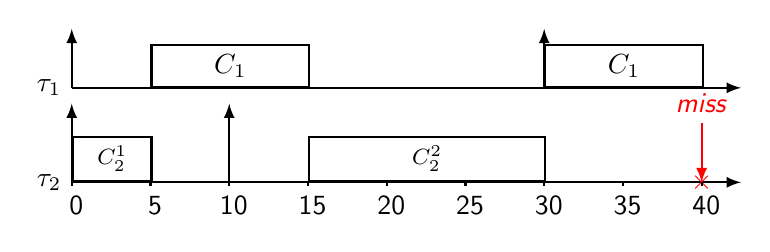
\begin{tikzpicture}[y=\uy, font=\sffamily,thick]
     
       
       
        \begin{scope}[shift={(0,0)}]
       \draw[->] (0,0)node[anchor=east,align=center] {$\tau_2$} -- coordinate (xaxis) (8.5,0);
      	\foreach \x in {3}{
      
	 	\node[task7, minimum width=6*\uy,
			anchor=south west] at ( \x, 0){\footnotesize $C_2^2$};
	}
	\foreach \x in {0}{

      		 \node[task7, minimum width=2*\uy,
anchor=south west] at ( \x, 0){\footnotesize $C_2^1$};
	 	
	}
	
	\foreach \x in {0}{
		\draw[->](\x,0) -- (\x,2)
	 		node[above] {};
	}
	\foreach \x in {2}{
		\draw[->](\x,0) -- (\x,2)
	 		node[above] {};
	}
	
	\foreach \x in {8}{
		\draw[->,red](\x,1.5) node[anchor=south] {\textit{miss}}  -- (\x,0)
			node[] {$\times$};
	 		
	}
	\foreach \x in {0,1,...,8}{
		\draw[-,below](\x,0) -- (\x,-0.1)
node[] {\pgfmathtruncatemacro\yi{5*\x} \yi};

			
	 		
	}
       \end{scope}
    
      \begin{scope}[shift={(0,2.4)}]
   
      	\draw[->](0,0) -- (0,1.5);
%\draw[->](2,0) -- (2,1);
\draw[->](6,0) -- (6,1.5);

	\foreach \x in {1,6}{
       		\node[task7, minimum width=4*\uy,
			anchor=south west] at ( \x, 0){$C_1$};
	 	
	}
	\draw[->] (0,0)node[anchor=east] {$\tau_1$} -- coordinate (xaxis) (8.5,0);


	
	
       \end{scope}
 %\draw[dotted] (10,0) -- (10,3.5);
    %  \draw[dotted] (15,0) -- (15,3.5);
     % \draw [<->] (10,3.5) -- (15,3.5)
     % 	node[anchor=south,pos=0.5] {$carry$-$in$};


      \end{tikzpicture}
	\end{sansmath}
	
\end{document}